% Options for packages loaded elsewhere
\PassOptionsToPackage{unicode}{hyperref}
\PassOptionsToPackage{hyphens}{url}
\PassOptionsToPackage{dvipsnames,svgnames,x11names}{xcolor}
%
\documentclass[
  letterpaper,
  DIV=11,
  numbers=noendperiod]{scrartcl}

\usepackage{amsmath,amssymb}
\usepackage{iftex}
\ifPDFTeX
  \usepackage[T1]{fontenc}
  \usepackage[utf8]{inputenc}
  \usepackage{textcomp} % provide euro and other symbols
\else % if luatex or xetex
  \usepackage{unicode-math}
  \defaultfontfeatures{Scale=MatchLowercase}
  \defaultfontfeatures[\rmfamily]{Ligatures=TeX,Scale=1}
\fi
\usepackage{lmodern}
\ifPDFTeX\else  
    % xetex/luatex font selection
\fi
% Use upquote if available, for straight quotes in verbatim environments
\IfFileExists{upquote.sty}{\usepackage{upquote}}{}
\IfFileExists{microtype.sty}{% use microtype if available
  \usepackage[]{microtype}
  \UseMicrotypeSet[protrusion]{basicmath} % disable protrusion for tt fonts
}{}
\makeatletter
\@ifundefined{KOMAClassName}{% if non-KOMA class
  \IfFileExists{parskip.sty}{%
    \usepackage{parskip}
  }{% else
    \setlength{\parindent}{0pt}
    \setlength{\parskip}{6pt plus 2pt minus 1pt}}
}{% if KOMA class
  \KOMAoptions{parskip=half}}
\makeatother
\usepackage{xcolor}
\setlength{\emergencystretch}{3em} % prevent overfull lines
\setcounter{secnumdepth}{5}
% Make \paragraph and \subparagraph free-standing
\makeatletter
\ifx\paragraph\undefined\else
  \let\oldparagraph\paragraph
  \renewcommand{\paragraph}{
    \@ifstar
      \xxxParagraphStar
      \xxxParagraphNoStar
  }
  \newcommand{\xxxParagraphStar}[1]{\oldparagraph*{#1}\mbox{}}
  \newcommand{\xxxParagraphNoStar}[1]{\oldparagraph{#1}\mbox{}}
\fi
\ifx\subparagraph\undefined\else
  \let\oldsubparagraph\subparagraph
  \renewcommand{\subparagraph}{
    \@ifstar
      \xxxSubParagraphStar
      \xxxSubParagraphNoStar
  }
  \newcommand{\xxxSubParagraphStar}[1]{\oldsubparagraph*{#1}\mbox{}}
  \newcommand{\xxxSubParagraphNoStar}[1]{\oldsubparagraph{#1}\mbox{}}
\fi
\makeatother

\usepackage{color}
\usepackage{fancyvrb}
\newcommand{\VerbBar}{|}
\newcommand{\VERB}{\Verb[commandchars=\\\{\}]}
\DefineVerbatimEnvironment{Highlighting}{Verbatim}{commandchars=\\\{\}}
% Add ',fontsize=\small' for more characters per line
\usepackage{framed}
\definecolor{shadecolor}{RGB}{241,243,245}
\newenvironment{Shaded}{\begin{snugshade}}{\end{snugshade}}
\newcommand{\AlertTok}[1]{\textcolor[rgb]{0.68,0.00,0.00}{#1}}
\newcommand{\AnnotationTok}[1]{\textcolor[rgb]{0.37,0.37,0.37}{#1}}
\newcommand{\AttributeTok}[1]{\textcolor[rgb]{0.40,0.45,0.13}{#1}}
\newcommand{\BaseNTok}[1]{\textcolor[rgb]{0.68,0.00,0.00}{#1}}
\newcommand{\BuiltInTok}[1]{\textcolor[rgb]{0.00,0.23,0.31}{#1}}
\newcommand{\CharTok}[1]{\textcolor[rgb]{0.13,0.47,0.30}{#1}}
\newcommand{\CommentTok}[1]{\textcolor[rgb]{0.37,0.37,0.37}{#1}}
\newcommand{\CommentVarTok}[1]{\textcolor[rgb]{0.37,0.37,0.37}{\textit{#1}}}
\newcommand{\ConstantTok}[1]{\textcolor[rgb]{0.56,0.35,0.01}{#1}}
\newcommand{\ControlFlowTok}[1]{\textcolor[rgb]{0.00,0.23,0.31}{\textbf{#1}}}
\newcommand{\DataTypeTok}[1]{\textcolor[rgb]{0.68,0.00,0.00}{#1}}
\newcommand{\DecValTok}[1]{\textcolor[rgb]{0.68,0.00,0.00}{#1}}
\newcommand{\DocumentationTok}[1]{\textcolor[rgb]{0.37,0.37,0.37}{\textit{#1}}}
\newcommand{\ErrorTok}[1]{\textcolor[rgb]{0.68,0.00,0.00}{#1}}
\newcommand{\ExtensionTok}[1]{\textcolor[rgb]{0.00,0.23,0.31}{#1}}
\newcommand{\FloatTok}[1]{\textcolor[rgb]{0.68,0.00,0.00}{#1}}
\newcommand{\FunctionTok}[1]{\textcolor[rgb]{0.28,0.35,0.67}{#1}}
\newcommand{\ImportTok}[1]{\textcolor[rgb]{0.00,0.46,0.62}{#1}}
\newcommand{\InformationTok}[1]{\textcolor[rgb]{0.37,0.37,0.37}{#1}}
\newcommand{\KeywordTok}[1]{\textcolor[rgb]{0.00,0.23,0.31}{\textbf{#1}}}
\newcommand{\NormalTok}[1]{\textcolor[rgb]{0.00,0.23,0.31}{#1}}
\newcommand{\OperatorTok}[1]{\textcolor[rgb]{0.37,0.37,0.37}{#1}}
\newcommand{\OtherTok}[1]{\textcolor[rgb]{0.00,0.23,0.31}{#1}}
\newcommand{\PreprocessorTok}[1]{\textcolor[rgb]{0.68,0.00,0.00}{#1}}
\newcommand{\RegionMarkerTok}[1]{\textcolor[rgb]{0.00,0.23,0.31}{#1}}
\newcommand{\SpecialCharTok}[1]{\textcolor[rgb]{0.37,0.37,0.37}{#1}}
\newcommand{\SpecialStringTok}[1]{\textcolor[rgb]{0.13,0.47,0.30}{#1}}
\newcommand{\StringTok}[1]{\textcolor[rgb]{0.13,0.47,0.30}{#1}}
\newcommand{\VariableTok}[1]{\textcolor[rgb]{0.07,0.07,0.07}{#1}}
\newcommand{\VerbatimStringTok}[1]{\textcolor[rgb]{0.13,0.47,0.30}{#1}}
\newcommand{\WarningTok}[1]{\textcolor[rgb]{0.37,0.37,0.37}{\textit{#1}}}

\providecommand{\tightlist}{%
  \setlength{\itemsep}{0pt}\setlength{\parskip}{0pt}}\usepackage{longtable,booktabs,array}
\usepackage{calc} % for calculating minipage widths
% Correct order of tables after \paragraph or \subparagraph
\usepackage{etoolbox}
\makeatletter
\patchcmd\longtable{\par}{\if@noskipsec\mbox{}\fi\par}{}{}
\makeatother
% Allow footnotes in longtable head/foot
\IfFileExists{footnotehyper.sty}{\usepackage{footnotehyper}}{\usepackage{footnote}}
\makesavenoteenv{longtable}
\usepackage{graphicx}
\makeatletter
\def\maxwidth{\ifdim\Gin@nat@width>\linewidth\linewidth\else\Gin@nat@width\fi}
\def\maxheight{\ifdim\Gin@nat@height>\textheight\textheight\else\Gin@nat@height\fi}
\makeatother
% Scale images if necessary, so that they will not overflow the page
% margins by default, and it is still possible to overwrite the defaults
% using explicit options in \includegraphics[width, height, ...]{}
\setkeys{Gin}{width=\maxwidth,height=\maxheight,keepaspectratio}
% Set default figure placement to htbp
\makeatletter
\def\fps@figure{htbp}
\makeatother

\KOMAoption{captions}{tableheading}
\makeatletter
\@ifpackageloaded{caption}{}{\usepackage{caption}}
\AtBeginDocument{%
\ifdefined\contentsname
  \renewcommand*\contentsname{Table of contents}
\else
  \newcommand\contentsname{Table of contents}
\fi
\ifdefined\listfigurename
  \renewcommand*\listfigurename{List of Figures}
\else
  \newcommand\listfigurename{List of Figures}
\fi
\ifdefined\listtablename
  \renewcommand*\listtablename{List of Tables}
\else
  \newcommand\listtablename{List of Tables}
\fi
\ifdefined\figurename
  \renewcommand*\figurename{Figure}
\else
  \newcommand\figurename{Figure}
\fi
\ifdefined\tablename
  \renewcommand*\tablename{Table}
\else
  \newcommand\tablename{Table}
\fi
}
\@ifpackageloaded{float}{}{\usepackage{float}}
\floatstyle{ruled}
\@ifundefined{c@chapter}{\newfloat{codelisting}{h}{lop}}{\newfloat{codelisting}{h}{lop}[chapter]}
\floatname{codelisting}{Listing}
\newcommand*\listoflistings{\listof{codelisting}{List of Listings}}
\makeatother
\makeatletter
\makeatother
\makeatletter
\@ifpackageloaded{caption}{}{\usepackage{caption}}
\@ifpackageloaded{subcaption}{}{\usepackage{subcaption}}
\makeatother

\ifLuaTeX
  \usepackage{selnolig}  % disable illegal ligatures
\fi
\usepackage{bookmark}

\IfFileExists{xurl.sty}{\usepackage{xurl}}{} % add URL line breaks if available
\urlstyle{same} % disable monospaced font for URLs
\hypersetup{
  pdftitle={McKinney Fire metabolism: Publication figures},
  pdfauthor={Laurel Genzoli},
  colorlinks=true,
  linkcolor={blue},
  filecolor={Maroon},
  citecolor={Blue},
  urlcolor={Blue},
  pdfcreator={LaTeX via pandoc}}


\title{McKinney Fire metabolism: Publication figures}
\author{Laurel Genzoli}
\date{2026-02-23}

\begin{document}
\maketitle

\renewcommand*\contentsname{Table of contents}
{
\hypersetup{linkcolor=}
\setcounter{tocdepth}{3}
\tableofcontents
}

\section{Script Description}\label{script-description}

This script make the publication plots for the first draft of the
McKinney Fire Metabolism paper, which is the report. Some plots were
post processed to lay out (figure 1).

\subsection{Load packages and data}\label{load-packages-and-data}

\subsubsection{Packages}\label{packages}

\begin{Shaded}
\begin{Highlighting}[]
\FunctionTok{setwd}\NormalTok{(}\StringTok{\textquotesingle{}/Users/laurelgenzoli/Dropbox/2024\_Projects/Mckinney\_Fire\_Metab/Mck{-}Fire{-}Metab{-}GH\textquotesingle{}}\NormalTok{)}


\FunctionTok{library}\NormalTok{(lubridate)}
\FunctionTok{library}\NormalTok{(dataRetrieval)}
\FunctionTok{library}\NormalTok{(viridis)}
\FunctionTok{library}\NormalTok{(cowplot)}
\FunctionTok{library}\NormalTok{(ggpubr)}
\FunctionTok{library}\NormalTok{(streamMetabolizer)}
\FunctionTok{library}\NormalTok{(hms)}
\FunctionTok{library}\NormalTok{(plotly)}
\FunctionTok{library}\NormalTok{(scales)}
\FunctionTok{library}\NormalTok{(data.table)}
\FunctionTok{library}\NormalTok{(zoo)}
\FunctionTok{library}\NormalTok{(nlme)}
\FunctionTok{library}\NormalTok{(tidyverse)}
\FunctionTok{library}\NormalTok{(magick)}
\FunctionTok{library}\NormalTok{(scales)}
\FunctionTok{library}\NormalTok{(ggbreak)}
\FunctionTok{library}\NormalTok{(brms)}
\FunctionTok{library}\NormalTok{(segmented)}
\FunctionTok{library}\NormalTok{(ggnewscale)}


\FunctionTok{theme\_set}\NormalTok{(}\FunctionTok{theme\_classic}\NormalTok{())}
\end{Highlighting}
\end{Shaded}

\subsection{Data}\label{data}

Data including both daily outputs and sub-daily/high frequency data.

\begin{Shaded}
\begin{Highlighting}[]
\DocumentationTok{\#\# Final metabolism data, with QA points turned to NA}
\NormalTok{met.mle.final }\OtherTok{\textless{}{-}} \FunctionTok{read\_csv}\NormalTok{(}\StringTok{"Data/met\_mle\_final.csv"}\NormalTok{) }\SpecialCharTok{\%\textgreater{}\%}
 \FunctionTok{mutate}\NormalTok{(}\AttributeTok{year =} \FunctionTok{as.factor}\NormalTok{(year),}
         \AttributeTok{fire =} \FunctionTok{factor}\NormalTok{(}\FunctionTok{ifelse}\NormalTok{(date }\SpecialCharTok{\textgreater{}} \StringTok{"2022{-}08{-}02"}\NormalTok{, }\StringTok{"After"}\NormalTok{, }\StringTok{"Before"}\NormalTok{),}
                       \AttributeTok{levels =} \FunctionTok{c}\NormalTok{(}\StringTok{"Before"}\NormalTok{, }\StringTok{"After"}\NormalTok{))) }\SpecialCharTok{\%\textgreater{}\%}
  \FunctionTok{mutate}\NormalTok{(}\AttributeTok{GPP =} \FunctionTok{ifelse}\NormalTok{(QA.code }\SpecialCharTok{==} \DecValTok{1}\NormalTok{, }\ConstantTok{NA}\NormalTok{, GPP))}\SpecialCharTok{\%\textgreater{}\%}
  \FunctionTok{mutate}\NormalTok{(}\AttributeTok{GPP.upper =} \FunctionTok{ifelse}\NormalTok{(QA.code }\SpecialCharTok{==} \DecValTok{1}\NormalTok{, }\ConstantTok{NA}\NormalTok{, GPP.upper))}\SpecialCharTok{\%\textgreater{}\%}
  \FunctionTok{mutate}\NormalTok{(}\AttributeTok{GPP.lower =} \FunctionTok{ifelse}\NormalTok{(QA.code }\SpecialCharTok{==} \DecValTok{1}\NormalTok{, }\ConstantTok{NA}\NormalTok{, GPP.lower))}\SpecialCharTok{\%\textgreater{}\%}
  \FunctionTok{mutate}\NormalTok{(}\AttributeTok{ER =} \FunctionTok{ifelse}\NormalTok{(QA.code }\SpecialCharTok{\%in\%} \FunctionTok{c}\NormalTok{(}\DecValTok{1}\NormalTok{,}\DecValTok{2}\NormalTok{), }\ConstantTok{NA}\NormalTok{, ER))}\SpecialCharTok{\%\textgreater{}\%}
  \FunctionTok{mutate}\NormalTok{(}\AttributeTok{ER.upper =} \FunctionTok{ifelse}\NormalTok{(QA.code }\SpecialCharTok{\%in\%} \FunctionTok{c}\NormalTok{(}\DecValTok{1}\NormalTok{,}\DecValTok{2}\NormalTok{), }\ConstantTok{NA}\NormalTok{, ER.upper))}\SpecialCharTok{\%\textgreater{}\%}
  \FunctionTok{mutate}\NormalTok{(}\AttributeTok{ER.lower =} \FunctionTok{ifelse}\NormalTok{(QA.code }\SpecialCharTok{\%in\%} \FunctionTok{c}\NormalTok{(}\DecValTok{1}\NormalTok{,}\DecValTok{2}\NormalTok{), }\ConstantTok{NA}\NormalTok{, ER.lower))}\SpecialCharTok{\%\textgreater{}\%}
  \FunctionTok{mutate}\NormalTok{(}\AttributeTok{NEP =} \FunctionTok{ifelse}\NormalTok{(}\FunctionTok{is.na}\NormalTok{(ER), }\ConstantTok{NA}\NormalTok{, NEP))}
  

\DocumentationTok{\#\# Final metabolism data day of pulse}
\NormalTok{met.mle.final.FIRE }\OtherTok{\textless{}{-}} \FunctionTok{read\_csv}\NormalTok{(}\StringTok{"Data/met\_mle\_final.csv"}\NormalTok{)}
  

\DocumentationTok{\#\# Data for sub{-}daily response plots during Fire}
\NormalTok{sub.day}\FloatTok{.1} \OtherTok{\textless{}{-}} \FunctionTok{read\_csv}\NormalTok{(}\StringTok{"Data/sub{-}daily{-}FIRE.csv"}\NormalTok{)}\SpecialCharTok{\%\textgreater{}\%}
  \FunctionTok{mutate}\NormalTok{(}\AttributeTok{datetime =} \FunctionTok{force\_tz}\NormalTok{(datetime, }\AttributeTok{tzone =} \StringTok{"Etc/GMT+7"}\NormalTok{))}


\DocumentationTok{\#\# model fit data used in SI turbidity spike plot}
\NormalTok{mod.fits.bin }\OtherTok{\textless{}{-}} \FunctionTok{read\_csv}\NormalTok{(}\StringTok{"Data/Metab\_Output/Binned/SV\_fits\_BIN.csv"}\NormalTok{)}\SpecialCharTok{\%\textgreater{}\%}
 \FunctionTok{mutate}\NormalTok{(}\AttributeTok{week =} \FunctionTok{week}\NormalTok{(solar.time))}\SpecialCharTok{\%\textgreater{}\%}
 \FunctionTok{mutate}\NormalTok{(}\AttributeTok{jday =} \FunctionTok{yday}\NormalTok{(solar.time),}
        \AttributeTok{year =} \FunctionTok{year}\NormalTok{(solar.time),}
        \AttributeTok{mon =} \FunctionTok{month}\NormalTok{ (solar.time),}
        \AttributeTok{DO.def =}\NormalTok{ DO.sat }\SpecialCharTok{{-}}\NormalTok{ DO.obs)}\SpecialCharTok{\%\textgreater{}\%}
   \FunctionTok{mutate}\NormalTok{(}\AttributeTok{solar.time =} \FunctionTok{force\_tz}\NormalTok{(solar.time, }\AttributeTok{tz =} \StringTok{"Etc/GMT+7"}\NormalTok{))}


\DocumentationTok{\#\# Sub daily turbidity: used in spike plots and in stats}
\DocumentationTok{\#\# This data is not included in the public GIT Release}
\DocumentationTok{\#\# Contact Karuk Tribe DNR for this data}

\NormalTok{hour.turb }\OtherTok{\textless{}{-}} \FunctionTok{read\_csv}\NormalTok{(}\StringTok{"Data/SV\_2018{-}2024\_AllParams.csv"}\NormalTok{, }
                      \AttributeTok{skip =} \DecValTok{16}\NormalTok{, }
                      \AttributeTok{col\_names =} \FunctionTok{c}\NormalTok{(}\StringTok{"dtime"}\NormalTok{, }\StringTok{"temp.water"}\NormalTok{, }\StringTok{"sc"}\NormalTok{, }\StringTok{"domg"}\NormalTok{, }\StringTok{"ph"}\NormalTok{, }\StringTok{"turb"}\NormalTok{)) }\SpecialCharTok{\%\textgreater{}\%}
  \FunctionTok{mutate}\NormalTok{(}\AttributeTok{dtime =} \FunctionTok{ymd\_hms}\NormalTok{(dtime)) }\SpecialCharTok{\%\textgreater{}\%}                 \CommentTok{\# convert to POSIXct}
  \FunctionTok{separate}\NormalTok{(dtime, }\AttributeTok{into =} \FunctionTok{c}\NormalTok{(}\StringTok{"date"}\NormalTok{, }\StringTok{"time"}\NormalTok{), }\AttributeTok{sep =} \StringTok{" "}\NormalTok{, }\AttributeTok{remove =}\NormalTok{ F) }\SpecialCharTok{\%\textgreater{}\%}
  \FunctionTok{mutate}\NormalTok{(}\AttributeTok{date =} \FunctionTok{as.Date}\NormalTok{(date),}
        \AttributeTok{datetime =} \FunctionTok{force\_tz}\NormalTok{(dtime, }\AttributeTok{tz =} \StringTok{"Etc/GMT+7"}\NormalTok{),}
         \AttributeTok{solar.time =}\NormalTok{ datetime) }\SpecialCharTok{\%\textgreater{}\%}                  \CommentTok{\# use the datetime column}
  \FunctionTok{filter}\NormalTok{(date }\SpecialCharTok{\textgreater{}=} \FunctionTok{as.Date}\NormalTok{(}\StringTok{"2022{-}07{-}30"}\NormalTok{)) }\SpecialCharTok{\%\textgreater{}\%}
\NormalTok{  dplyr}\SpecialCharTok{::}\FunctionTok{select}\NormalTok{(solar.time, turb)}


\NormalTok{hour.turb.all }\OtherTok{\textless{}{-}} \FunctionTok{read\_csv}\NormalTok{(}\StringTok{"Data/SV\_2018{-}2024\_AllParams.csv"}\NormalTok{, }
                      \AttributeTok{skip =} \DecValTok{16}\NormalTok{, }
                      \AttributeTok{col\_names =} \FunctionTok{c}\NormalTok{(}\StringTok{"dtime"}\NormalTok{, }\StringTok{"temp.water"}\NormalTok{, }\StringTok{"sc"}\NormalTok{, }\StringTok{"domg"}\NormalTok{, }\StringTok{"ph"}\NormalTok{, }\StringTok{"turb"}\NormalTok{)) }\SpecialCharTok{\%\textgreater{}\%}
  \FunctionTok{mutate}\NormalTok{(}\AttributeTok{dtime =} \FunctionTok{ymd\_hms}\NormalTok{(dtime)) }\SpecialCharTok{\%\textgreater{}\%}                 \CommentTok{\# convert to POSIXct}
  \FunctionTok{separate}\NormalTok{(dtime, }\AttributeTok{into =} \FunctionTok{c}\NormalTok{(}\StringTok{"date"}\NormalTok{, }\StringTok{"time"}\NormalTok{), }\AttributeTok{sep =} \StringTok{" "}\NormalTok{, }\AttributeTok{remove =}\NormalTok{ F) }\SpecialCharTok{\%\textgreater{}\%}
  \FunctionTok{mutate}\NormalTok{(}\AttributeTok{date =} \FunctionTok{as.Date}\NormalTok{(date),}
        \AttributeTok{datetime =} \FunctionTok{force\_tz}\NormalTok{(dtime, }\AttributeTok{tz =} \StringTok{"Etc/GMT+7"}\NormalTok{),}
         \AttributeTok{solar.time =}\NormalTok{ datetime) }\SpecialCharTok{\%\textgreater{}\%}                  \CommentTok{\# use the datetime column}
\NormalTok{  dplyr}\SpecialCharTok{::}\FunctionTok{select}\NormalTok{(solar.time, turb)}
\end{Highlighting}
\end{Shaded}

\section{Figures for main manuscript}\label{figures-for-main-manuscript}

\subsection{Figure 1: During the storm
panel}\label{figure-1-during-the-storm-panel}

\begin{itemize}
\tightlist
\item
  Instantaneous light, flow, turb, DO for 6 days
\item
  To plot below with the map and photos of event
\item
  1 sub-panel for each parameter
\end{itemize}

\small

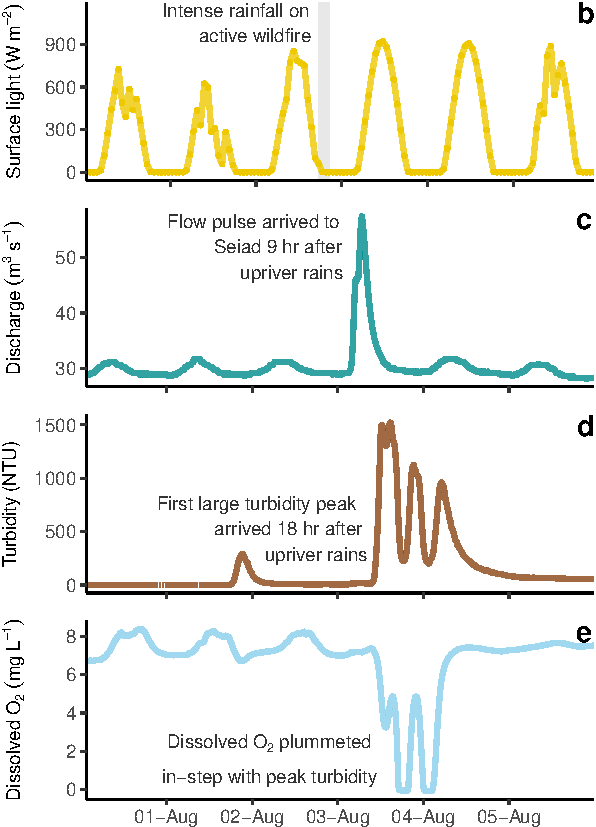
\includegraphics{Final_Figures_files/figure-pdf/unnamed-chunk-3-1.pdf}

\normalsize

\subsection{Figure 2: Full time series showing change after
fire}\label{figure-2-full-time-series-showing-change-after-fire}

\subsubsection{Left panels, time series of light, flow, turb and
metabolism}\label{left-panels-time-series-of-light-flow-turb-and-metabolism}

\small

\begin{verbatim}
[1] Before After 
Levels: Before After
\end{verbatim}

\normalsize

\subsubsection{Calc mean here:}\label{calc-mean-here}

This is just raw data means--not sure why I did this here. I have a
table of the means from the model that were calc in the Stats script.

\small

\begin{verbatim}
# A tibble: 12 x 5
   var         fire      mean   lower   upper
   <chr>       <fct>    <dbl>   <dbl>   <dbl>
 1 ER          Before  -7.46   -7.71   -7.21 
 2 ER          After   -3.81   -4.03   -3.60 
 3 GHI.day     Before 207.    202.    213.   
 4 GHI.day     After  187.    177.    196.   
 5 GPP         Before   8.70    8.43    8.96 
 6 GPP         After    3.29    3.05    3.53 
 7 NEP         Before   1.75    1.63    1.88 
 8 NEP         After   -0.503  -0.658  -0.347
 9 SV.cms      Before  55.1    53.0    57.3  
10 SV.cms      After   60.6    56.3    64.9  
11 turb_median Before   3.69    3.52    3.86 
12 turb_median After   18.2    12.6    23.7  
\end{verbatim}

\normalsize

\subsubsection{Right panel, means and laying out the final
plot}\label{right-panel-means-and-laying-out-the-final-plot}

The data frames for this plot are in the ``Stats\_D1\_Report.qmd''
Script. This plot will not run here without running the models in the
Stats script first. Need to run these in unison, but the script is long
and the model takes a while to run so I didn't want it to clutter this
script.

\small

\normalsize

\subsection{Figure 3}\label{figure-3}

\subsubsection{Figure 3 panel A: Turbidity by
discharge}\label{figure-3-panel-a-turbidity-by-discharge}

\begin{itemize}
\tightlist
\item
  Run the model
\item
  Then, run the figure (next code chunk)
\end{itemize}

Not a variable slope/variable intercept (this is a random effect with
groups) like I originally coded it; what we have is an interaction model
(outcomes changed little, but good to use the correct model structure).

\[T = \beta_0 + \beta_1 \times F + \beta_2 \times Q + \beta_3 \times F \times Q + \epsilon\]

\small

\normalsize

\small

\normalsize

\subsubsection{Figure 3 Panel E}\label{figure-3-panel-e}

\begin{itemize}
\tightlist
\item
  This is the GLM segmented (breakpoint) model
\item
  This figure will not run without the model being run in the Stats
  script
\item
  Prediction lines are for Jan and July conditions, based on pre and
  post fire years
\end{itemize}

\paragraph{GLM model for turb to DO}\label{glm-model-for-turb-to-do}

\begin{itemize}
\tightlist
\item
  Additional model specs are in the Models script
\item
  Running this here allows the plot below to render using just this
  script
\end{itemize}

\small

\normalsize

\paragraph{Break point plot}\label{break-point-plot}

\small

\normalsize

\subsubsection{Figure 3 panes B-D, and final
layout}\label{figure-3-panes-b-d-and-final-layout}

\small

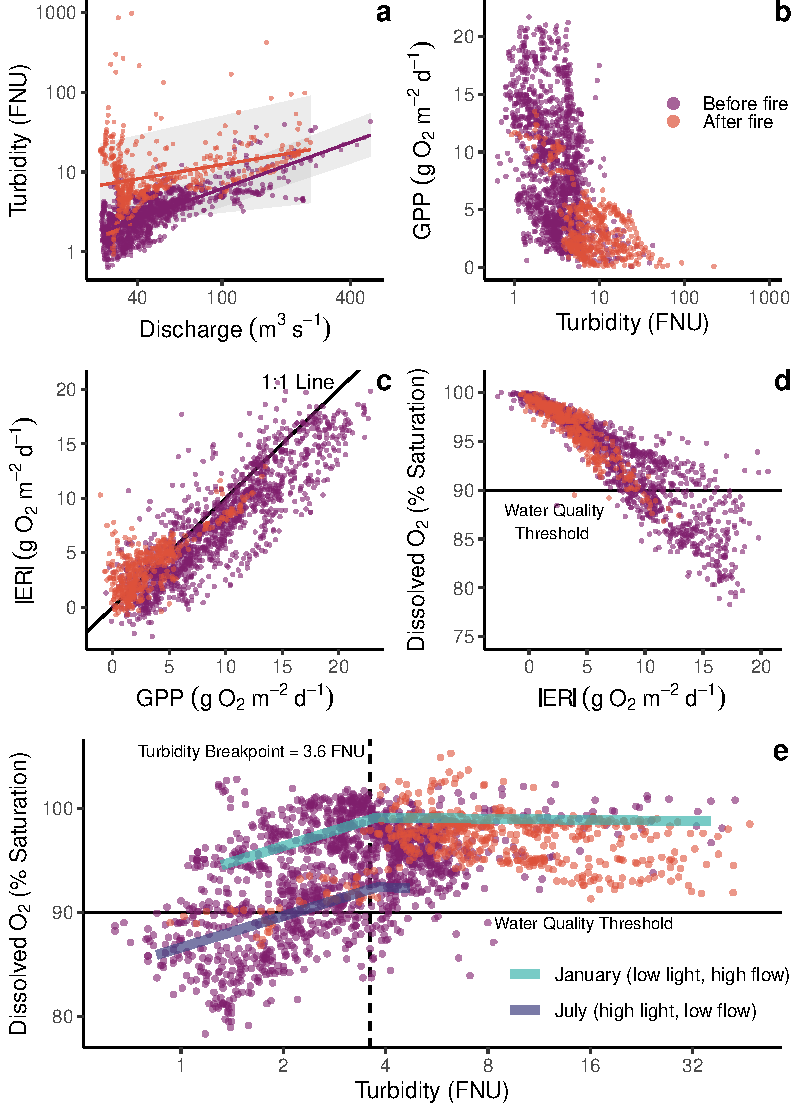
\includegraphics{Final_Figures_files/figure-pdf/unnamed-chunk-11-1.pdf}

\normalsize

\section{Suppliment Figures}\label{suppliment-figures}

Figures S1 and S2 were pulled from the depth script and the metabolism
output script.

\subsection{Figure S3: Full metab data
set}\label{figure-s3-full-metab-data-set}

\small

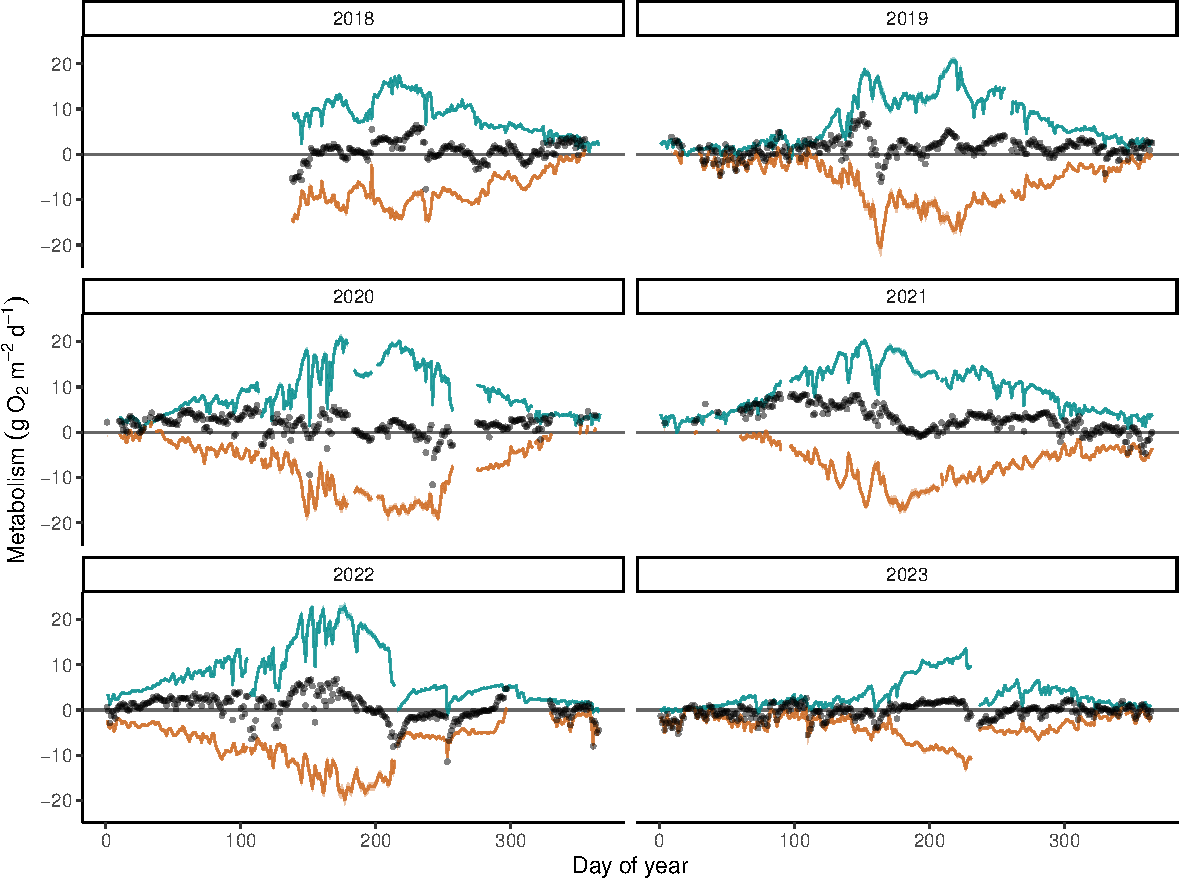
\includegraphics{Final_Figures_files/figure-pdf/unnamed-chunk-12-1.pdf}

\normalsize

\subsection{Figure S4: full metab data set for the \textasciitilde month
around the time of the
fire}\label{figure-s4-full-metab-data-set-for-the-month-around-the-time-of-the-fire}

2 wks before and 2 wks after fire

\small

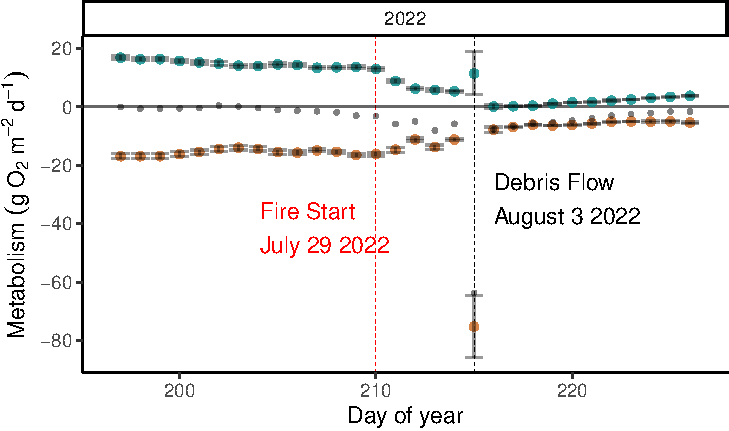
\includegraphics{Final_Figures_files/figure-pdf/unnamed-chunk-13-1.pdf}

\normalsize

\subsection{Figure S5 GPP x ER}\label{figure-s5-gpp-x-er}

\small

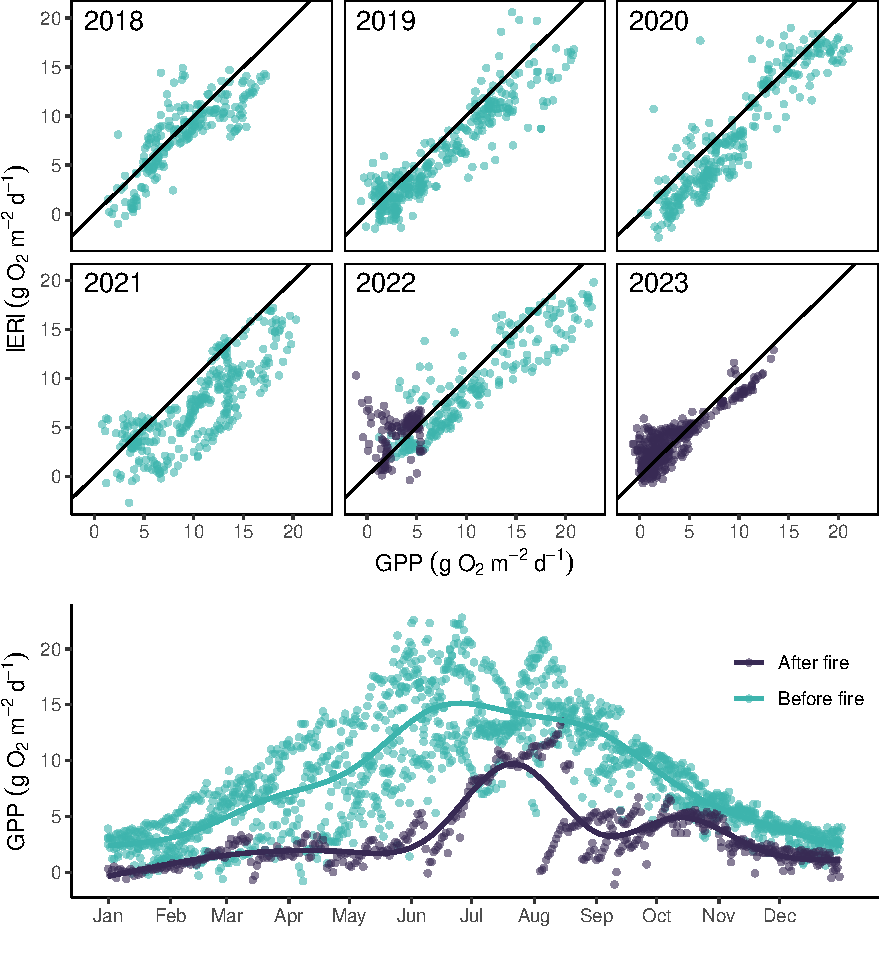
\includegraphics{Final_Figures_files/figure-pdf/unnamed-chunk-14-1.pdf}

\normalsize

\subsection{Figure S6: DO during turbidity
spikes}\label{figure-s6-do-during-turbidity-spikes}

\subsubsection{Middle panel: show the Turb spikes post
fire}\label{middle-panel-show-the-turb-spikes-post-fire}

\begin{itemize}
\tightlist
\item
  Panel showing daily median turbidity following the fire
\item
  Numbers show spikes over 50; these are the ``events''
\item
  Post processed number placement in pdf editor
\end{itemize}

\small

\normalsize

\subsubsection{And the DO plots for each
``event''}\label{and-the-do-plots-for-each-event}

\paragraph{Data prep first}\label{data-prep-first}

\begin{itemize}
\tightlist
\item
  There are two sets of plots
\item
  One goes above the turbidity time series, one below
\item
  Plots were a total hack to get turbidity and DO on same panel
\item
  I had to select the ``windows''--3 days--of high turbidity events
\item
  Then, select the hourly data from the metab model output
\item
  And, the turbidity sub-daily data
\end{itemize}

\small

\normalsize

\paragraph{Set of 4 top panels:}\label{set-of-4-top-panels}

\small

\normalsize

\paragraph{Set of 4 bottom panels:}\label{set-of-4-bottom-panels}

\small

\normalsize

\paragraph{Put all plots together for this overly complex
figure}\label{put-all-plots-together-for-this-overly-complex-figure}

\small

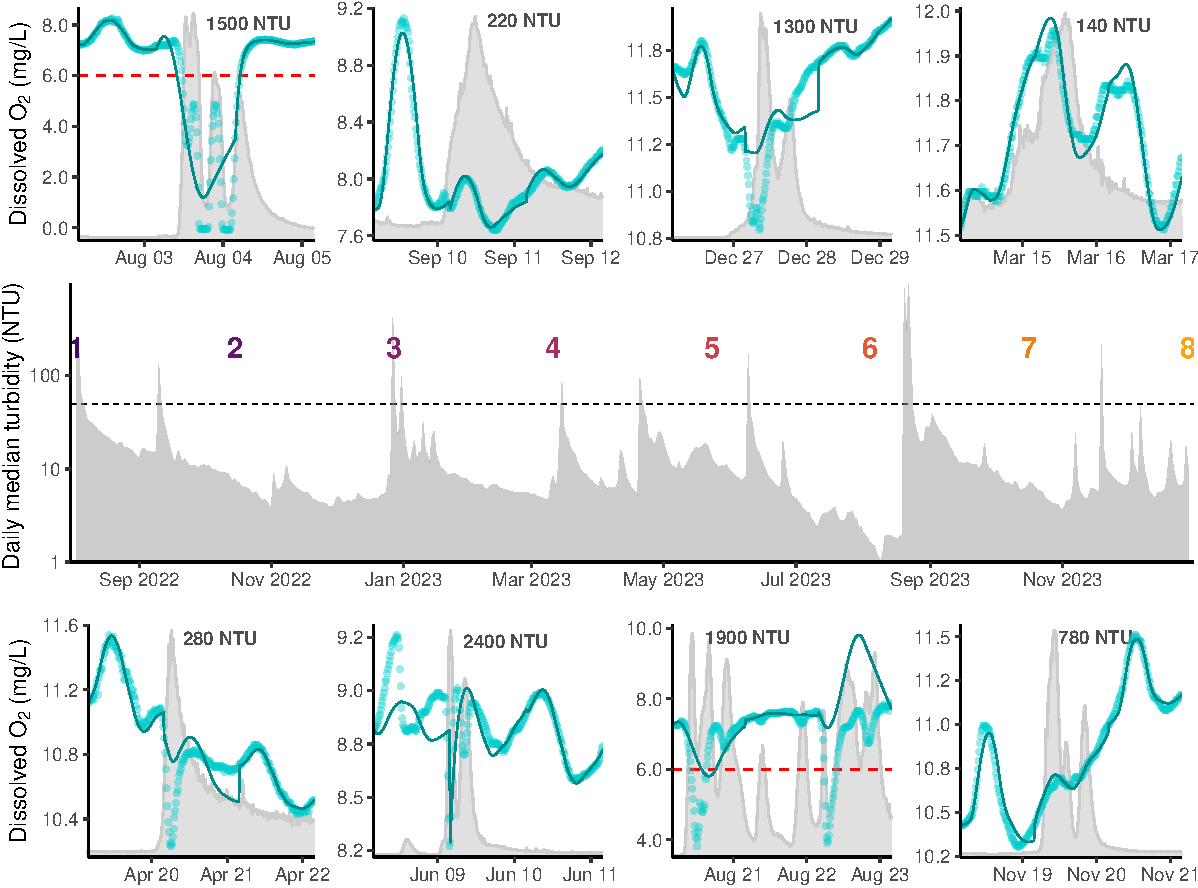
\includegraphics{Final_Figures_files/figure-pdf/unnamed-chunk-19-1.pdf}

\normalsize

\subsection{Figure S7: GPP by Flow, Turb, and
LIght}\label{figure-s7-gpp-by-flow-turb-and-light}

\small

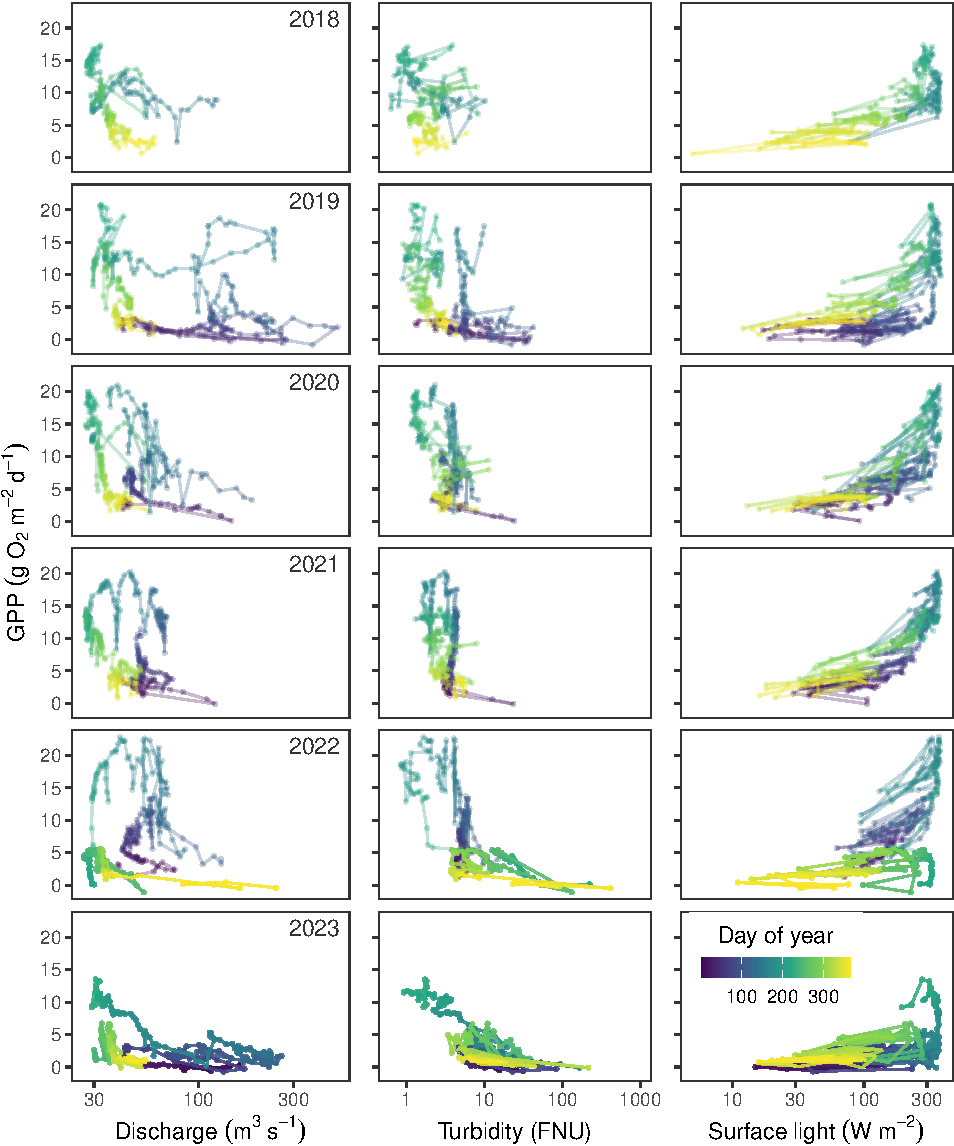
\includegraphics{Final_Figures_files/figure-pdf/unnamed-chunk-20-1.pdf}

\normalsize

\subsection{Figure S8: DO min and
MEtabolism}\label{figure-s8-do-min-and-metabolism}

\small

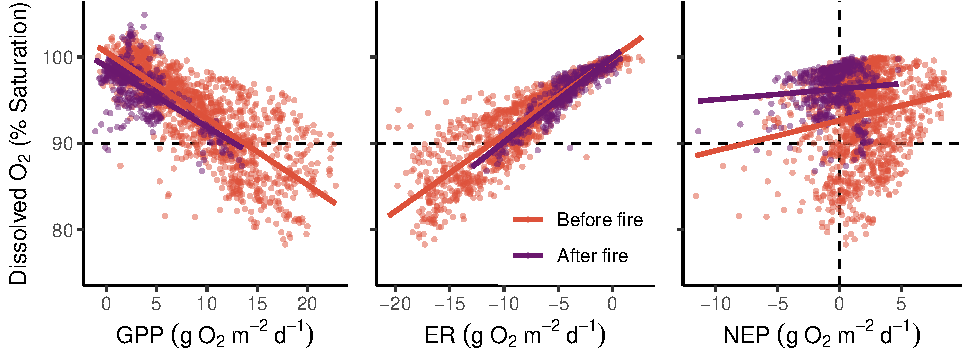
\includegraphics{Final_Figures_files/figure-pdf/unnamed-chunk-21-1.pdf}

\normalsize




\end{document}
